\documentclass[10pt]{article}\usepackage[]{graphicx}\usepackage[]{color}
%% maxwidth is the original width if it is less than linewidth
%% otherwise use linewidth (to make sure the graphics do not exceed the margin)
\makeatletter
\def\maxwidth{ %
  \ifdim\Gin@nat@width>\linewidth
    \linewidth
  \else
    \Gin@nat@width
  \fi
}
\makeatother

\definecolor{fgcolor}{rgb}{0.345, 0.345, 0.345}
\newcommand{\hlnum}[1]{\textcolor[rgb]{0.686,0.059,0.569}{#1}}%
\newcommand{\hlstr}[1]{\textcolor[rgb]{0.192,0.494,0.8}{#1}}%
\newcommand{\hlcom}[1]{\textcolor[rgb]{0.678,0.584,0.686}{\textit{#1}}}%
\newcommand{\hlopt}[1]{\textcolor[rgb]{0,0,0}{#1}}%
\newcommand{\hlstd}[1]{\textcolor[rgb]{0.345,0.345,0.345}{#1}}%
\newcommand{\hlkwa}[1]{\textcolor[rgb]{0.161,0.373,0.58}{\textbf{#1}}}%
\newcommand{\hlkwb}[1]{\textcolor[rgb]{0.69,0.353,0.396}{#1}}%
\newcommand{\hlkwc}[1]{\textcolor[rgb]{0.333,0.667,0.333}{#1}}%
\newcommand{\hlkwd}[1]{\textcolor[rgb]{0.737,0.353,0.396}{\textbf{#1}}}%
\let\hlipl\hlkwb

\usepackage{framed}
\makeatletter
\newenvironment{kframe}{%
 \def\at@end@of@kframe{}%
 \ifinner\ifhmode%
  \def\at@end@of@kframe{\end{minipage}}%
  \begin{minipage}{\columnwidth}%
 \fi\fi%
 \def\FrameCommand##1{\hskip\@totalleftmargin \hskip-\fboxsep
 \colorbox{shadecolor}{##1}\hskip-\fboxsep
     % There is no \\@totalrightmargin, so:
     \hskip-\linewidth \hskip-\@totalleftmargin \hskip\columnwidth}%
 \MakeFramed {\advance\hsize-\width
   \@totalleftmargin\z@ \linewidth\hsize
   \@setminipage}}%
 {\par\unskip\endMakeFramed%
 \at@end@of@kframe}
\makeatother

\definecolor{shadecolor}{rgb}{.97, .97, .97}
\definecolor{messagecolor}{rgb}{0, 0, 0}
\definecolor{warningcolor}{rgb}{1, 0, 1}
\definecolor{errorcolor}{rgb}{1, 0, 0}
\newenvironment{knitrout}{}{} % an empty environment to be redefined in TeX

\usepackage{alltt}
\usepackage{amssymb, amsmath, amsthm, verbatim, layout, setspace, graphicx, float, geometry}
\usepackage{tabularx}
\usepackage{booktabs}

\newcommand{\textnote}[1]{\textbf{\textit{#1}}}
\newcommand{\code}[1]{\textbf{\textit{#1}}}
\newcommand{\grad}{\nabla}
\newcommand\inv[1]{#1\raisebox{1.15ex}{$\scriptscriptstyle-\!1$}}

% ------ layout ------
\IfFileExists{upquote.sty}{\usepackage{upquote}}{}
\begin{document}
\title{Linear Regression: Part 2}
\author{Jeremy Oldfather}
\maketitle







\subsection*{Multiple Linear Regression - Last Time }

When we regress $y$ on more than one independent variable, say ($x_1, x_2,...,x_k$) rather than simply ($x_1$), the regression framework is referred to as {\bf multiple linear regression}.

What might motivate us to introduce multiple regressors? One reason might be that we have reason to suspect {\bf omitted variable bias}. In order for our model to be subject to omitted variable bias, we must have both of the following problems:

\begin{description}
  \item [$E(y|x_1,x_2) \ne E(y|x_1) $] :  Meaning our expectation about the dependent variable $y$ changes when we include the additional independent variable. If $E(y|x_1,x_2) = E(y|x_1)$, we would say that $y$ is conditionally independent of $x_2$---meaning either $x_2$ is completely irrevelant to predicting $y$, or that any information contained in $x_2$ is already contained in $x_1$.
  \item [$Cor(x_1, x_2) \ne 0 $] :  Meaning the additional variable $x_2$ must be correlated with a current dependent variable $x_1$.
\end{description}

For example, when we plot the distribution of residuals from our previous model by neighborhood, we can see that the variable {\bf neighborhood} meets the first critera for omitted variable bias since for Anacostia we would consistently overstate the impact of a change in living area on the change in sales price.

\begin{knitrout}\small
\definecolor{shadecolor}{rgb}{0.969, 0.969, 0.969}\color{fgcolor}\begin{kframe}
\begin{alltt}
\hlstd{selected.nhoods}\hlkwb{<-}\hlkwd{c}\hlstd{(}\hlstr{"FOGGY BOTTOM"}\hlstd{,}\hlstr{"ANACOSTIA"}\hlstd{,}\hlstr{"LEDROIT PARK"}\hlstd{,}\hlstr{"TAKOMA"}\hlstd{,}\hlstr{"GEORGETOWN"}\hlstd{)}
\hlkwd{data.frame}\hlstd{(}\hlkwc{e}\hlstd{=}\hlkwd{resid}\hlstd{(fit),}\hlkwc{g}\hlstd{=data.model}\hlopt{$}\hlstd{neighborhood)} \hlopt
  \hlkwd{filter}\hlstd{(g} \hlopt \hlstd{selected.nhoods)} \hlopt
  \hlkwd{ggplot}\hlstd{(}\hlkwd{aes}\hlstd{(}\hlkwc{y}\hlstd{=e,}\hlkwc{x}\hlstd{=g))} \hlopt{+} \hlkwd{geom_boxplot}\hlstd{()}
\end{alltt}
\end{kframe}

{\centering 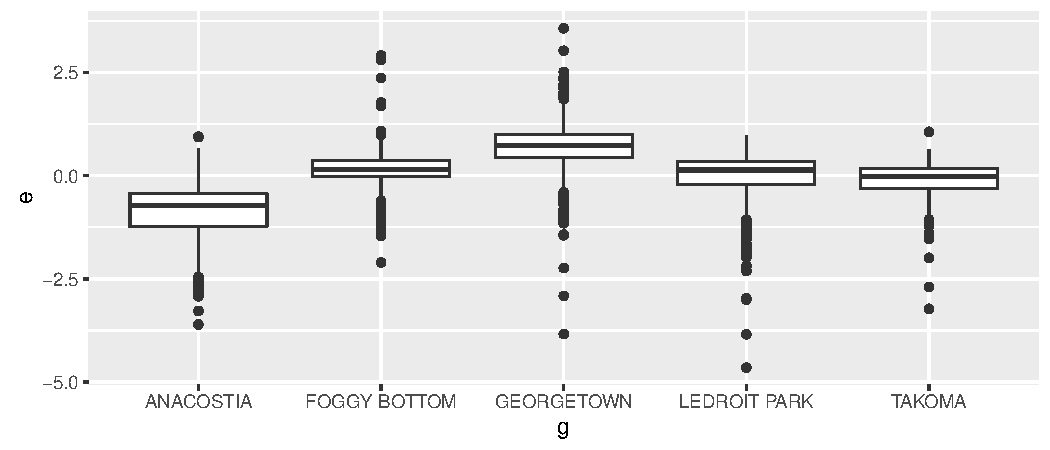
\includegraphics[width=\maxwidth]{figure/boxplot_residuals-1} 

}



\end{knitrout}

To check the second criteria, that $Cor(living\_area,neighborhood) \ne 0$, we can plug a dummy variable for each neighborhood into R's {\bf cor()} function.

\begin{knitrout}\small
\definecolor{shadecolor}{rgb}{0.969, 0.969, 0.969}\color{fgcolor}\begin{kframe}
\begin{alltt}
\hlkwd{cor}\hlstd{(data.model}\hlopt{$}\hlstd{log_living_sqft,data.model}\hlopt{$}\hlstd{neighborhood}\hlopt{==}\hlstr{"ANACOSTIA"}\hlstd{)}
\end{alltt}
\begin{verbatim}
## [1] 0.02040842
\end{verbatim}
\begin{alltt}
\hlkwd{cor}\hlstd{(data.model}\hlopt{$}\hlstd{log_living_sqft,data.model}\hlopt{$}\hlstd{neighborhood}\hlopt{==}\hlstr{"FOGGY BOTTOM"}\hlstd{)}
\end{alltt}
\begin{verbatim}
## [1] -0.1058928
\end{verbatim}
\begin{alltt}
\hlkwd{cor}\hlstd{(data.model}\hlopt{$}\hlstd{log_living_sqft,data.model}\hlopt{$}\hlstd{neighborhood}\hlopt{==}\hlstr{"GEORGETOWN"}\hlstd{)}
\end{alltt}
\begin{verbatim}
## [1] 0.06697943
\end{verbatim}
\begin{alltt}
\hlkwd{cor}\hlstd{(data.model}\hlopt{$}\hlstd{log_living_sqft,data.model}\hlopt{$}\hlstd{neighborhood}\hlopt{==}\hlstr{"LEDROIT PARK"}\hlstd{)}
\end{alltt}
\begin{verbatim}
## [1] 0.03272786
\end{verbatim}
\begin{alltt}
\hlkwd{cor}\hlstd{(data.model}\hlopt{$}\hlstd{log_living_sqft,data.model}\hlopt{$}\hlstd{neighborhood}\hlopt{==}\hlstr{"TAKOMA"}\hlstd{)}
\end{alltt}
\begin{verbatim}
## [1] 0.0146363
\end{verbatim}
\end{kframe}
\end{knitrout}

Anacostia, Ledroit Park, and Takoma are either weakly or not at all correlated with living area, but Foggy Bottom is negatively correlated and Georgetown is weakly positively correlated.

To see the connection between including these neighborhoods in the regression, I will create a new variable that sets all other neighborhoods to "other". I put "aa" at the beginning because R treats the first element of a factor variable as the base value for the regression. So by doing this, we can see how the neighborhoods we analyzed above affect our regression in terms of all other DC neighborhoods.

\begin{knitrout}\small
\definecolor{shadecolor}{rgb}{0.969, 0.969, 0.969}\color{fgcolor}\begin{kframe}
\begin{alltt}
\hlstd{fit2}\hlkwb{<-}\hlstd{data.model} \hlopt
  \hlkwd{mutate}\hlstd{(}\hlkwc{nhoods5}\hlstd{=}\hlkwd{ifelse}\hlstd{(neighborhood} \hlopt \hlstd{selected.nhoods,}
                        \hlstd{neighborhood,}
                        \hlstr{"aa_other"}\hlstd{)}
         \hlstd{)} \hlopt
  \hlkwd{lm}\hlstd{(log_sale_price} \hlopt{~} \hlstd{log_living_sqft} \hlopt{+} \hlkwd{factor}\hlstd{(nhoods5),}\hlkwc{data}\hlstd{=.)}
\hlkwd{summary}\hlstd{(fit2)}
\end{alltt}
\begin{verbatim}
## 
## Call:
## lm(formula = log_sale_price ~ log_living_sqft + factor(nhoods5), 
##     data = .)
## 
## Residuals:
##      Min       1Q   Median       3Q      Max 
## -13.6024  -0.3463   0.1282   0.4260   6.5927 
## 
## Coefficients:
##                              Estimate Std. Error t value Pr(>|t|)    
## (Intercept)                  7.913192   0.033502 236.204  < 2e-16 ***
## log_living_sqft              0.699649   0.004723 148.133  < 2e-16 ***
## factor(nhoods5)ANACOSTIA    -0.832172   0.023094 -36.034  < 2e-16 ***
## factor(nhoods5)FOGGY BOTTOM  0.192594   0.024741   7.784 7.09e-15 ***
## factor(nhoods5)GEORGETOWN    0.715779   0.015717  45.543  < 2e-16 ***
## factor(nhoods5)LEDROIT PARK -0.007375   0.022117  -0.333 0.738790    
## factor(nhoods5)TAKOMA       -0.129247   0.036654  -3.526 0.000422 ***
## ---
## Signif. codes:  0 '***' 0.001 '**' 0.01 '*' 0.05 '.' 0.1 ' ' 1
## 
## Residual standard error: 0.7052 on 85290 degrees of freedom
## Multiple R-squared:  0.2355,	Adjusted R-squared:  0.2354 
## F-statistic:  4378 on 6 and 85290 DF,  p-value: < 2.2e-16
\end{verbatim}
\end{kframe}
\end{knitrout}

Comparing the coefficients for each neighborhood with the distribution of their residuals in the boxplot above, we can see the pattern. The coefficient for a dummy shifts our fitted line up or down by the amount of the coefficient.  For example, when all the dummies are turned off (equal zero), 

\begin{align*}
 \hat{y}_i &= 7.913192 + 0.699649 x_i
\end{align*}

But when Anacostia equals 1,

\begin{align*}
\hat{y}_i &= 7.913192 + 0.699649 x_i - 0.832172(1) \\
  &= 7.08102 + 0.699649 x_i
\end{align*}

Now I will add dummies for the rest of the DC neighborhoods and run the regression again.

\begin{knitrout}\small
\definecolor{shadecolor}{rgb}{0.969, 0.969, 0.969}\color{fgcolor}\begin{kframe}
\begin{alltt}
\hlstd{fit3}\hlkwb{<-}\hlkwd{lm}\hlstd{(log_sale_price} \hlopt{~} \hlstd{log_living_sqft} \hlopt{+} \hlkwd{factor}\hlstd{(neighborhood),}\hlkwc{data}\hlstd{=data.model)}
\hlkwd{coef}\hlstd{(fit3)[}\hlnum{1}\hlopt{:}\hlnum{2}\hlstd{]}
\end{alltt}
\begin{verbatim}
##     (Intercept) log_living_sqft 
##        7.634167        0.716211
\end{verbatim}
\begin{alltt}
\hlkwd{summary}\hlstd{(}\hlkwd{resid}\hlstd{(fit3))}
\end{alltt}
\begin{verbatim}
##      Min.   1st Qu.    Median      Mean   3rd Qu.      Max. 
## -13.33000  -0.22140   0.07746   0.00000   0.29570   6.22800
\end{verbatim}
\end{kframe}
\end{knitrout}

\subsection*{Multiple Linear Regression - Continuation }

Previously, we showed how to fit a line using simple linear regression (one regressor) and then how adding relevant regressors to our model can improve the fit and limit omitted variable bias. We used a box-plot to show that residuals were correlated with a variable that was not yet included in our model. However, we did not discuss how we can prove to ourselves in a rigorous way that the goodness-of-fit in the second model is better than the one in the first.

\subsubsection*{Goodness-of-Fit ($R^2$)}

Let's start by returning to our definition of the sum of squared residuals. We can re-write it in terms of the residuals in the following way.

\begin{align}
SSR(\beta_0,...,\beta_k) &= \sum_i ( y_i -  (\beta_0 + \beta_1 x_{i1} + \cdots + \beta_k x_{ik} ) )^2 \\
 &= \sum_i ( y_i -  (\hat{y}_i ) )^2 \\
 &= \sum_i  ( \epsilon_i - 0  )^2 \\
 &= (n-1) Var(\epsilon) 
\end{align}

Written this way, we can see that the sum of squared residuals is proportional to the variation of the residuals. In other words, {\bf SSR is the variation in house prices that our model does not explain}. 

It turns out that we can also write down a formula for the variation in house prices that our model does explain, the { \bf{explained sum of squares (SSE)}}, as well as one for the total variation in house prices, or {\bf{total sum of squares (SST)}}. 

\begin{align}
SSR(\beta_0,...,\beta_k) &= \sum_i  ( \epsilon_i - 0  )^2 = (n-1) Var(\epsilon) \\
SSE(\beta_0,...,\beta_k) &= \sum_i  ( \hat{y}_i - \bar{y} )^2 = (n-1) Var(\hat{y}) \\
SST &= \sum_i  ( y_i - \bar{y} )^2 = (n-1) Var(y) 
\end{align}

Together, these components of variation have the following relationship:

\begin{align}
SST &= SSE + SSR
\end{align}

With this in mind, $R^2$ can be defined as either the share of total variation explained by the model,

\begin{align}
R^2 &= \frac{SSE}{SST} \\
&= \frac{Var(\hat{y})}{Var(y)} 
\end{align}

Or as 1 minus the share of total variation unexplain by the model,

\begin{align}
R^2 &= 1 - \frac{SSR}{SST} \\
&= 1 -\frac{Var(\epsilon)}{Var(y)} 
\end{align}

Let's calculate the R-squared for a model and compare it to the regression output of R.

\begin{knitrout}\small
\definecolor{shadecolor}{rgb}{0.969, 0.969, 0.969}\color{fgcolor}\begin{kframe}
\begin{alltt}
\hlcom{# fit the simple model}
\hlstd{fit}\hlkwb{<-}\hlkwd{lm}\hlstd{(log_sale_price} \hlopt{~} \hlstd{log_living_sqft,}\hlkwc{data}\hlstd{=data.model)}

\hlcom{# calculate R-squared}
\hlnum{1}\hlopt{-}\hlkwd{var}\hlstd{(}\hlkwd{resid}\hlstd{(fit))}\hlopt{/}\hlkwd{var}\hlstd{(data.model}\hlopt{$}\hlstd{log_sale_price)}
\end{alltt}
\begin{verbatim}
## [1] 0.2039985
\end{verbatim}
\begin{alltt}
\hlcom{# compare to the regression output}
\hlkwd{summary}\hlstd{(fit)}
\end{alltt}
\begin{verbatim}
## 
## Call:
## lm(formula = log_sale_price ~ log_living_sqft, data = data.model)
## 
## Residuals:
##      Min       1Q   Median       3Q      Max 
## -13.6189  -0.3601   0.1332   0.4313   6.5902 
## 
## Coefficients:
##                 Estimate Std. Error t value Pr(>|t|)    
## (Intercept)     7.875186   0.033900   232.3   <2e-16 ***
## log_living_sqft 0.706351   0.004778   147.8   <2e-16 ***
## ---
## Signif. codes:  0 '***' 0.001 '**' 0.01 '*' 0.05 '.' 0.1 ' ' 1
## 
## Residual standard error: 0.7196 on 85295 degrees of freedom
## Multiple R-squared:  0.204,	Adjusted R-squared:  0.204 
## F-statistic: 2.186e+04 on 1 and 85295 DF,  p-value: < 2.2e-16
\end{verbatim}
\end{kframe}
\end{knitrout}

The regression output refers to $R^2$ as "multiple R-squared", which is simply an allusion to $R^2$ under the multiple linear regression framework---it is still calculated as described above.

{\bf Adjusted R-squared}, however, is different from $R^2$. $R^2$ does not account for the number of regressors being added to the model. So for small datasets, $R^2$ will always increase slightly regardless of the explanatory power of the variable being added to the model. Adjusted R-squared takes the number of added regressors into account and makes the necessary adjustment.

\subsubsection*{Model Selection}

Many methods are available for comparing and selecting the best model (from a statistical perspective). 

For the following examples, let's consider two models. The first is called our { \bf restricted model}. It is our best model so far that will act as our base model. The second is called our {\bf unrestricted model}. This is our new model that we would like to test against the first. Let's estimate these models now from the house price data:

\begin{knitrout}\small
\definecolor{shadecolor}{rgb}{0.969, 0.969, 0.969}\color{fgcolor}\begin{kframe}
\begin{alltt}
\hlstd{fit.res}\hlkwb{<-}\hlkwd{lm}\hlstd{(log_sale_price} \hlopt{~} \hlstd{log_living_sqft,}\hlkwc{data}\hlstd{=data.model)}
\hlstd{fit.unres}\hlkwb{<-}\hlkwd{lm}\hlstd{(log_sale_price} \hlopt{~} \hlstd{log_living_sqft} \hlopt{+} \hlkwd{factor}\hlstd{(neighborhood),}\hlkwc{data}\hlstd{=data.model)}
\end{alltt}
\end{kframe}
\end{knitrout}

\subsubsection*{Testing Adjusted R-squared ($\bar{R}^2$)}

Comparing the Adjusted R-squared of two model specifications is a popular method of choosing one model over another.

If $\bar{R}^2_{unres} > \bar{R}^2_{res}$, then we reject the hypothesis that the unrestricted model containing no explanatory power over the restricted one. Then the unstricted model becomes our new basis for comparison. 

Let's try this test on our house price models.

\begin{knitrout}\small
\definecolor{shadecolor}{rgb}{0.969, 0.969, 0.969}\color{fgcolor}\begin{kframe}
\begin{alltt}
\hlkwd{summary}\hlstd{(fit.res)}\hlopt{$}\hlstd{adj.r.squared}
\end{alltt}
\begin{verbatim}
## [1] 0.2039892
\end{verbatim}
\begin{alltt}
\hlkwd{summary}\hlstd{(fit.unres)}\hlopt{$}\hlstd{adj.r.squared}
\end{alltt}
\begin{verbatim}
## [1] 0.4656749
\end{verbatim}
\end{kframe}
\end{knitrout}

In this example, we would reject the hypothesis that the model including the neighborhood dummies contains no explanatory power beyond that of the restricted model without the dummies.

\subsubsection*{F-test}

In general, an F-test is used to test to the equivalence of variances for two normal distributions. Since well-specified linear regression models will have residuals that are normally distributed (we have not dicussed this), the F-test is commonly used to test the equivalence of the unexplained variation between two models.

For this test, we calculate an F-statistic from the SSR of both models and compared it to the critical value from the F-distribution. For the number of regressors in each respective model ($p$), and the number of observations ($n$), the F-statistic is defined as:

\begin{align}
F &= \frac{SSR_{res} - SSR_{unres}}{p_{unres} - p_{res}} \bigg{/} \frac{SSR_{unres}}{n - p_{unres}}
\end{align}

This F-statistic has the distribution $F(p_{unres} - p_{res}, n - p_{unres})$. The critical value is then chosen from this distribution based on the desired significance level (usually .05).

Let's try this test on our house price models.

\begin{knitrout}\small
\definecolor{shadecolor}{rgb}{0.969, 0.969, 0.969}\color{fgcolor}\begin{kframe}
\begin{alltt}
\hlkwd{anova}\hlstd{(fit.res,fit.unres)}
\end{alltt}
\begin{verbatim}
## Analysis of Variance Table
## 
## Model 1: log_sale_price ~ log_living_sqft
## Model 2: log_sale_price ~ log_living_sqft + factor(neighborhood)
##   Res.Df   RSS Df Sum of Sq      F    Pr(>F)    
## 1  85295 44166                                  
## 2  85241 29628 54     14538 774.58 < 2.2e-16 ***
## ---
## Signif. codes:  0 '***' 0.001 '**' 0.01 '*' 0.05 '.' 0.1 ' ' 1
\end{verbatim}
\end{kframe}
\end{knitrout}

Again, we would reject the hypothesis that the model including the neighborhood dummies contains no explanatory power beyond that of the restricted model without the dummies.

However, notice that the F-test provides us with a degree of confidence for rejecting the restricted model. It also shows the number of regressor that were added in the unstricted model-- the neighborhood factor results in 54 dummies being added.

\subsubsection*{Other Methods for Model Selection}

Other methods exist for model selection, but will not be covered here. You can read more about them on wikipedia or in your favorite statistics / ecomometrics textbook. Some of the more popular ones are the Likelihood Ratio test (LR), Akaike information criterio (AIC), and the Bayesian informaiton criterion (BIC).

\subsection*{Generalized Linear Models (GLM)  }

For the oridinary least squares (OLS) regression framework above, we were able to describe the fitted values $\hat{y}_i$ as the expected value of $y_i$ given our regressors ($x_i$) and the estimated betas ($\hat{\beta}$):

\begin{align}
  \hat{y}_i = E(y_i|\hat{\beta};x_i) \label{ols_expectation}
\end{align}

The generalized linear model (GLM) framework expands upon OLS by allowing for the response variable ($y$) to be of a wider range of distributions. To do this, we allow for inclusion of a {\bf link function} that we will call $g$. However, in following the notation in Equation \ref{ols_expectation} above, we will reference its inverse, $\inv{g}$. 

\begin{align}
  \hat{y}_i = E(y_i|\inv{g},\hat{\beta};x_i)
\end{align}

The link function is that which connects $\hat{y}_i$ to $E(y_i|\beta;x_i)$. For example, if $g(z)=ln(z)$, then $\inv{g}(z)=e^z$ and

\begin{align}
  ln(\hat{y}_i) &= E(y_i|\hat{\beta};x_i) \\
  &= \hat{\beta}_0 + \hat{\beta}_1 x_{i1} + \cdots + \hat{\beta}_1 x_{ik} \\
  \hat{y}_i &= E(y_i|e^z,\beta;x_i) \\
  &= e^{\hat{\beta}_0 + \hat{\beta}_1 x_{i1} + \cdots + \hat{\beta}_1 x_{ik}}
\end{align}

Then our loss function (analogous to SSR but a more general) can be stated as:

\begin{align}
   \hat{\beta} = \underset{\beta}{argmin} \; ||y_i - E(y_i|\inv{g},\beta;x_i)||
\end{align}

It not important, in terms of this class, to know how this loss function is minimized. However, you should know that, unlike the SSR in OLS, this loss function does not always have a closed-form solution. So GLM models can take much longer to estimate than OLS models.

\subsubsection*{GLM Families}

With the {\bf glm()} function provided by R, we can estimate GLM models just like we did with {\bf lm()}, we only need to provide the family and link function so it knows the type of response we are trying to model. 

I will show examples of the gaussian (normal), logistic, and poisson regression. However, the R documentation for {\bf glm()} provides a full list of possible models and the wikipedia page for "generalized linear models" has a great overview table of the possible models.

\subsubsection*{Gaussian (identity)}

\begin{tabularx}{\textwidth}{r@{}l@{}}
  { Distribution of $y$ } &: Normal \\
  { Link Function } &: $g(z)=z$ \\
  { Inverse Function } &: $\inv{g}(z)=z$ \\
\end{tabularx}

\vspace{2ex}
\hspace*{\fill}%

Notice that because the link is the identity, the GLM gaussian model ends up taking the same form as the OLS regression.

\begin{align}
  \hat{y}_i &= E(y_i|\inv{g},\hat{\beta};x_i) \\
  &= E(y_i|z,\hat{\beta};x_i) \\
  &= \hat{\beta}_0 + \hat{\beta}_1 x_{i1} + \cdots + \hat{\beta}_1 x_{ik}
\end{align}

We can estimate GLM version of our house price model as follows:

\begin{knitrout}\small
\definecolor{shadecolor}{rgb}{0.969, 0.969, 0.969}\color{fgcolor}\begin{kframe}
\begin{alltt}
\hlstd{fit.gaussian}\hlkwb{<-}\hlkwd{glm}\hlstd{(log_sale_price} \hlopt{~} \hlstd{log_living_sqft,}
                  \hlkwc{data}\hlstd{=data.model,}
                  \hlkwc{family}\hlstd{=}\hlkwd{gaussian}\hlstd{(}\hlkwc{link}\hlstd{=}\hlstr{"identity"}\hlstd{))}
\hlkwd{summary}\hlstd{(fit.gaussian)}
\end{alltt}
\begin{verbatim}
## 
## Call:
## glm(formula = log_sale_price ~ log_living_sqft, family = gaussian(link = "identity"), 
##     data = data.model)
## 
## Deviance Residuals: 
##      Min        1Q    Median        3Q       Max  
## -13.6189   -0.3601    0.1332    0.4313    6.5902  
## 
## Coefficients:
##                 Estimate Std. Error t value Pr(>|t|)    
## (Intercept)     7.875186   0.033900   232.3   <2e-16 ***
## log_living_sqft 0.706351   0.004778   147.8   <2e-16 ***
## ---
## Signif. codes:  0 '***' 0.001 '**' 0.01 '*' 0.05 '.' 0.1 ' ' 1
## 
## (Dispersion parameter for gaussian family taken to be 0.5178044)
## 
##     Null deviance: 55485  on 85296  degrees of freedom
## Residual deviance: 44166  on 85295  degrees of freedom
## AIC: 185928
## 
## Number of Fisher Scoring iterations: 2
\end{verbatim}
\end{kframe}
\end{knitrout}


\subsubsection*{Binomial (logit)}

\begin{tabularx}{\textwidth}{r@{}l@{}}
  { Distribution of $y$ } &: Binomial \\
  { Link Function } &: $g(z)=ln( z / (1-z))$ \\
  { Inverse Function } &: $\inv{g}(z)= exp(z) / (1+exp(z)) $ \\
\end{tabularx}

\begin{align}
  \hat{y}_i &= E(y_i|\inv{g},\hat{\beta};x_i) \\
  &= E(y_i| \frac{exp(z)}{1+exp(z)},\hat{\beta};x_i) \\
  &= \frac{exp(\hat{\beta}_0 + \hat{\beta}_1 x_{i1} + \cdots + \hat{\beta}_1 x_{ik})}{1+exp(\hat{\beta}_0 + \hat{\beta}_1 x_{i1} + \cdots + \hat{\beta}_1 x_{ik})}
\end{align}

To test this model, we need some data that contains responses that represent successes and failures. Classification type problems can be framed in these terms if we consider one class to be a success and all other classes to be failures.

R provides a toy dataset called "iris" that it famously used to introduce classification. It contains observations on the sepal width/length and petal width/length of 3 species of iris. 

Let's create a response variable that is 1 if the species is "setosa" and 0 otherwise, and then fit a model with one of the observed variables.

\begin{knitrout}\small
\definecolor{shadecolor}{rgb}{0.969, 0.969, 0.969}\color{fgcolor}\begin{kframe}
\begin{alltt}
\hlkwd{data}\hlstd{(}\hlstr{"iris"}\hlstd{)}
\hlstd{iris}\hlkwb{<-}\hlstd{iris} \hlopt \hlkwd{mutate}\hlstd{(}\hlkwc{is.setosa}\hlstd{=}\hlkwd{ifelse}\hlstd{(Species}\hlopt{==}\hlstr{"setosa"}\hlstd{,}\hlnum{1}\hlstd{,}\hlnum{0}\hlstd{))}
\hlstd{fit.logit}\hlkwb{<-}\hlkwd{glm}\hlstd{(is.setosa} \hlopt{~} \hlstd{Sepal.Length,}
               \hlkwc{data}\hlstd{=iris,}
               \hlkwc{family}\hlstd{=}\hlkwd{binomial}\hlstd{(}\hlkwc{link}\hlstd{=}\hlstr{"logit"}\hlstd{))}
\hlkwd{summary}\hlstd{(fit.logit)}
\end{alltt}
\begin{verbatim}
## 
## Call:
## glm(formula = is.setosa ~ Sepal.Length, family = binomial(link = "logit"), 
##     data = iris)
## 
## Deviance Residuals: 
##      Min        1Q    Median        3Q       Max  
## -2.25787  -0.27914  -0.04605   0.31399   2.14316  
## 
## Coefficients:
##              Estimate Std. Error z value Pr(>|z|)    
## (Intercept)   27.8285     4.8276   5.765 8.19e-09 ***
## Sepal.Length  -5.1757     0.8934  -5.793 6.90e-09 ***
## ---
## Signif. codes:  0 '***' 0.001 '**' 0.01 '*' 0.05 '.' 0.1 ' ' 1
## 
## (Dispersion parameter for binomial family taken to be 1)
## 
##     Null deviance: 190.954  on 149  degrees of freedom
## Residual deviance:  71.836  on 148  degrees of freedom
## AIC: 75.836
## 
## Number of Fisher Scoring iterations: 7
\end{verbatim}
\end{kframe}
\end{knitrout}

The coefficients of the logistic regression can be interpretted as $\beta$ change in log-odds of a success with a 1 unit increase in the variable of interest.

What are log-odds? Well the odds of a success are defined as: 

$$odds = \frac{p(success)}{p(failure)}$$ 

So the log-odds is simply the odds on log-scale: 

\begin{align}
  log(odds) &= log\bigg(\frac{p(success)}{p(failure)}\bigg) \\
            &= log(p(success)) - log(p(failure))
\end{align}

For example, the probability of drawing a setosa from the dataset at random is $p=.33$. So the odds of drawing a setosa are $.33/.67=.5$ and the log-odds are $log(.33)-log(.67)=-0.69$

\subsubsection*{Poisson (log)}

\begin{tabularx}{\textwidth}{r@{}l@{}}
  { Distribution of $y$ } &: Poisson \\
  { Link Function } &: $g(z)=ln(z)$ \\
  { Inverse Function } &: $\inv{g}(z)= exp(z) $ \\
\end{tabularx}

\begin{align}
  \hat{y}_i &= E(y_i|\inv{g},\hat{\beta};x_i) \\
  &= E(y_i|exp(z),\hat{\beta};x_i) \\
  &= exp(\hat{\beta}_0 + \hat{\beta}_1 x_{i1} + \cdots + \hat{\beta}_1 x_{ik})
\end{align}

The Poisson allows us to estimate response variables that represent counts over a fix period of time. 

For example, I have some Uber logins for a specific geographic region. The original dataset is simply a vector of timestamps captured for 4 months. The data shown below have been aggregated to 15 minute intervals and show the cycles of logins for each day of the week.

\begin{knitrout}\small
\definecolor{shadecolor}{rgb}{0.969, 0.969, 0.969}\color{fgcolor}

{\centering 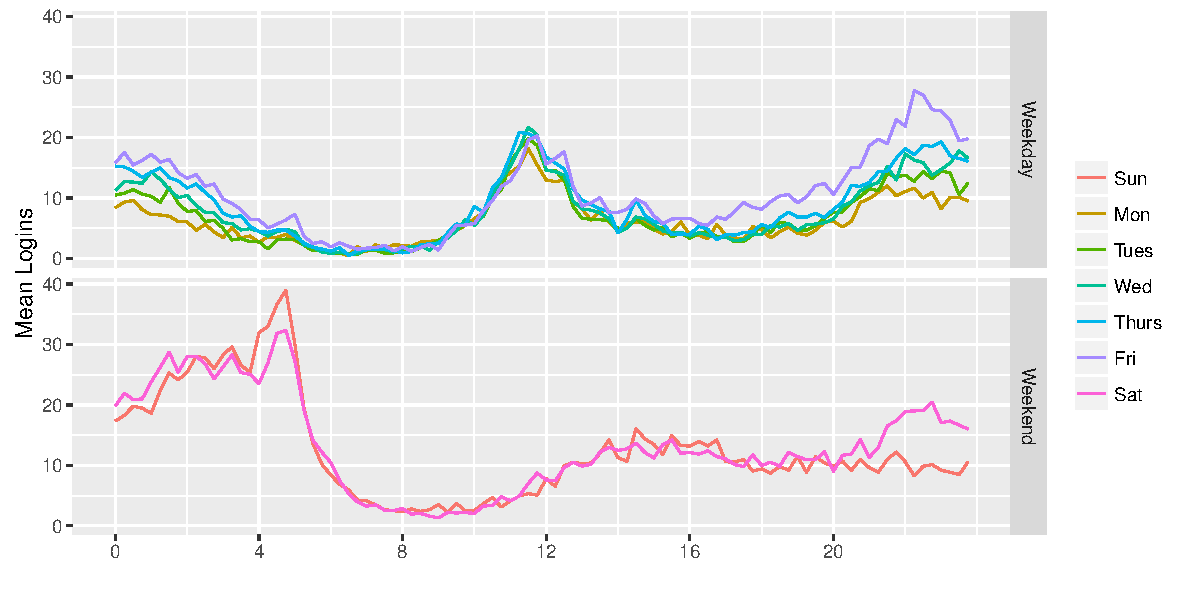
\includegraphics[width=\maxwidth]{figure/p2_daily_cycle-1} 

}



\end{knitrout}

Let's try to write down a model that captures the difference in behavior between the weekdays and weekends.

\begin{knitrout}\small
\definecolor{shadecolor}{rgb}{0.969, 0.969, 0.969}\color{fgcolor}\begin{kframe}
\begin{alltt}
\hlstd{logins15}\hlkwb{<-}\hlstd{logins15} \hlopt
  \hlkwd{mutate}\hlstd{(}\hlkwc{split}\hlstd{=}\hlkwd{ifelse}\hlstd{((wday}\hlopt{==}\hlstr{"Sun"} \hlopt{|} \hlstd{wday}\hlopt{==}\hlstr{"Sat"}\hlstd{),}\hlstr{"Weekend"}\hlstd{,}\hlstr{"Weekday"}\hlstd{) )}
\hlstd{fit.poisson}\hlkwb{<-}\hlkwd{glm}\hlstd{(log} \hlopt{~} \hlkwd{factor}\hlstd{(split)} \hlopt{+} \hlkwd{factor}\hlstd{(h)} \hlopt{+} \hlkwd{factor}\hlstd{(split)}\hlopt{:}\hlkwd{factor}\hlstd{(h) ,}
                 \hlkwc{data}\hlstd{=logins15,}
                 \hlkwc{family}\hlstd{=}\hlkwd{poisson}\hlstd{(}\hlkwc{link}\hlstd{=}\hlstr{"log"}\hlstd{))}
\end{alltt}
\end{kframe}
\end{knitrout}

The model above takes into consideration the weekday/weekend split, the hour of the day, and the interaction of the two together. Now let's test the model and see how many logins it predicts for an average {\bf weekend at 4am} and for an average {\bf weekday at 7am}.

\begin{knitrout}\small
\definecolor{shadecolor}{rgb}{0.969, 0.969, 0.969}\color{fgcolor}\begin{kframe}
\begin{alltt}
\hlkwd{predict}\hlstd{(fit.poisson,}
  \hlkwc{newdata}\hlstd{=}\hlkwd{data.frame}\hlstd{(}\hlkwc{split}\hlstd{=}\hlkwd{c}\hlstd{(}\hlstr{"Weekend"}\hlstd{,}\hlstr{"Weekday"}\hlstd{),}\hlkwc{h}\hlstd{=}\hlkwd{c}\hlstd{(}\hlnum{4}\hlstd{,}\hlnum{7}\hlstd{)),}
  \hlkwc{type}\hlstd{=}\hlstr{"response"}\hlstd{)}
\end{alltt}
\begin{verbatim}
##         1         2 
## 31.883333  1.545139
\end{verbatim}
\end{kframe}
\end{knitrout}

\end{document}
